\documentclass[journal, a4paper]{IEEEtran}

\usepackage{graphicx}   
\usepackage{hyperref} 
\usepackage{url}        
\usepackage{amssymb}
\usepackage{amsmath}    
\usepackage{booktabs} % Essential for nice tabs (see https://people.inf.ethz.ch/markusp/teaching/guides/guide-tables.pdf)
\usepackage{xcolor} 

\usepackage{bm}
\newcommand{\vect}[1]{\boldsymbol{\mathbf{#1}}}

% Some useful/example abbreviations for writing math
\newcommand{\argmax}{\operatornamewithlimits{argmax}}
\newcommand{\argmin}{\operatornamewithlimits{argmin}}
\newcommand{\x}{\mathbf{x}}
\newcommand{\y}{\mathbf{y}}
\newcommand{\ypred}{\mathbf{\hat y}}
\newcommand{\yp}{{\hat y}}

\newif\ifanonymous
\anonymoustrue

\begin{document}

% Define document title, do NOT write author names for the initial submission
\title{QuoridorRL: solving a two-player strategy game with reinforcement learning}
\ifanonymous
\author{Anonymous Authors}
\else
\author{Nathan Pollet, Rebecca Jaubert, Laura Minkova, Erwan Umlil and Clément Jambon}
\fi
\maketitle

% Write abstract here
\begin{abstract}
Quoridor is a zero-sum two-player board game which has not been extensively studied yet in the context of reinforcement learning. Its relatively large state and branching complexities and the lack of human-generated data make it very challenging and unsuitable for simple control strategies and exhaustive tree search approaches. Consequently, we provide a full \textit{gym}-like environment of the game and its mechanics. We then introduce three strategies with the aim of reaching human-level control: first a heuristic approach with \textit{MinMax} tree search relying on handcrafted evaluation functions, then a \textit{Monte-Carlo Tree Search} with \textit{Rapid Action Value Estimation} and finally a \textit{Monte-Carlo Tree Search} augmented with an evaluation neural network directly inspired from \textit{AlphaZero}. Even though, we have not reached convincing results yet, we are confident such approaches could yield satisfying performances with more computational resources.
\end{abstract}

% Each section begins with a \section{title} command
\section{Introduction}
\label{sec:intro}

In this project game theory, and in particular Zero-sum two-player game (RL) approaches, are considered through the concrete example of Quoridor, a complex strategy game designed by Mirko Marchesi and published by Gigamic Games \cite{quoridor-gigamic}. This is a particularly interesting use case as the game complexity is extremely large, 

 \textcolor{blue}{
- Why important? = Normally, use MinMax + heuristics but here, very large complexity, not much work before, 
- What challenges? = no human knowledge/pre-existing game data (contrary to Go, Shogi or Chess which have already been widely studied) => we cannot use supervised learning approaches (such as AlphaGo\cite{alphago}) / large state space, large branching spaces which bound exhaustive tree search methods to failure (e.g MinMax/AlphaBetaPruning)
- => heuristics, MC-RAVE (Rapid Action Value Estimation), AlphaZero (self-play+evaluation network to guide the expansion of the MCTS)
- Our model still training due to the large complexity, and trouble tuning the hyperparameters, especially for alphazero
Add qualification regarding conventional algorithms = DQN, PPO}



In addition to this paper, we provide the sources of our code at \footnote{Source: \url{}} and instructions to run each pipeline in the attached \textit{README} file. 

In the following, we first review prior approaches to provide robust and human-level control agents in two-player games with large complexities (section \ref{sec:background}), then we describe our implementation of the environment (section \ref{sec:environment}) and the models we used to solve it (section \ref{sec:models}), followed lastly by our experiments and resulting discussion (section \ref{sec:results}).

\section{Background and Related Work}
\label{sec:background}

\subsection{Game and complexity}
\label{ssec:complexity}
Describe the state and branching complexity of the game.
% https://math.stackexchange.com/questions/953750/counting-all-possible-board-positions-in-quoridor
% https://project.dke.maastrichtuniversity.nl/games/files/bsc/Mertens_BSc-paper.pdf

\subsection{MCTS}
\label{ssec:mcts}
Use paper Erwan \cite{mc-rave}

For a review of MCTS methods, refer to \cite{mcts-review}.

\subsection{Training without human knowledge}
\label{ssec:human-knowledge}

As seen in paragraph \ref{ssec:complexity}, \textit{Quoridor} is a game with very high state and branching complexities. Consequently, given the existing computational resources and considering that a decision must be provided by our agent in a moderately realistic amount of time, we cannot perform an exhaustive tree search such as MinMax. Therefore, we turned to an \textit{AlphaGo} approach as presented in \cite{alphago}.

In order to perform Monte-Carlo Tree Search over the large complexity space of \textit{Quoridor} and considering the lack of game data contrary to well-known and already analysed, we faced the challenge of training our model without human knowledge. To this extent, we turned to the \textit{"self-play"} approach initially presented in  \textit{AlphaGoZero}\cite{alphagozero} and later expanded to a larger set of games (namely Chess and Shogi) in \textit{AlphaZero}\cite{alphazero}. Furthermore, unlike \textit{AlphaGo}, \textit{AlphaZero} does not require handcrafted features and is thus more suited to the problem of solving a new game from scratch, as its neural network learns itself to capture features through residual convolutions of the game board. 

\section{Environment}
\label{sec:environment}

 \textit{Quoridor} being a little-known board game, there is, to our knowledge, no public implementation of its mechanics for the purpose of training RL agents. As a consequence, we provide with this project a turn-based environment with a \textit{gym}-like (cf. \cite{openai-gym})

As an introduction = environment set up from scratch => coding the came logics + choose consistent state and action spaces representations (and/or) wrapper

In order to limit the computational burden due to the very large complexity of the game in its original configuration, we chose to simplify the state space by restricting ourselves to the following rules:
\begin{itemize}
    \item the board has size $5\times 5$ (instead of $9\times 9$)
    \item each player can add at most $5$ walls (instead of $10$)
    \item the game can last at most $100$ turns, after which it is considered a "draw"
\end{itemize}

\subsection{Logic and representation}
\label{ssec:game-logic}

Although the game logic could be implemented by relying on a graph as suggested in \cite{heuristic-agent}, we chose a different intrinsic representation to limit the memory and computational footprint which are critical for efficient \textit{Monte Carlo Tree Searches}. We coded the game logic from scratch and provide an interface that allows users to check whether an action is valid or not, fetch all valid actions, take actions based on abstract representation or the string representation mentioned below. In order to check valid actions, we use the well-known $A^*$ algorithm (see chapter 3 of \cite{russel2010} for more details) in order to perform pathfinding. Note that every time we test an action, a pathfinding is performed even though little changes on the board have occured from one state to the other ; we should thus consider in future works a more robust solutions leveraging previous computations.

Intrinsiquely, the state $s\in\mathcal{S}$ of the game is represented as the set of player positions on the board, the number of remaining walls for each player, the index of the current player and a 2D array storing walls located by their lower left-hand positions and where $-1, 0, 1$ stands respectively for empty, horizontal ($x$-aligned), vertical ($y$-aligned).

States and actions can also be represented in a \textit{string} notation. Ours is inspired from the algebraic notation presented in \cite{quoridor-wikipedia}. More precisely, the $x$-coordinate of states are indexed in $\{1, \ldots, grid\_ size\}$ while the $y$-coordinate of states are indexed in $\{a, b, c, \ldots\}$. Walls are described in a similar fashion by appending the direction ($h$ for horizontal and $v$ for vertical) to the number-letter position couple. As such, we can represent player actions by the target \textit{string} position when the player performs a pawn move or the target wall position with the direction suffix when the player adds a wall. For completeness, we add the number of used walls to the state and the current player at the end of the \textit{string} representation. Equation \ref{eq:state-str} provides an example of such a representation and is illustrated in figure \ref{fig:state-str}.
\begin{equation}
    \label{eq:state-str}
    % 1d;5c;1dv;2bh;3av;3bv;4dv;p0:2;p1:3;p0;
    \underbrace{\text{1d;5c;}}_\text{pawn positions}\overbrace{\text{1dv;2bh;3av;3bv;4dv;}}^\text{walls}\underbrace{\text{p0:2;p1:3;}}_\text{used walls}\overbrace{\text{p0;}}^\text{current player}
\end{equation}
\begin{figure}
    \centering
    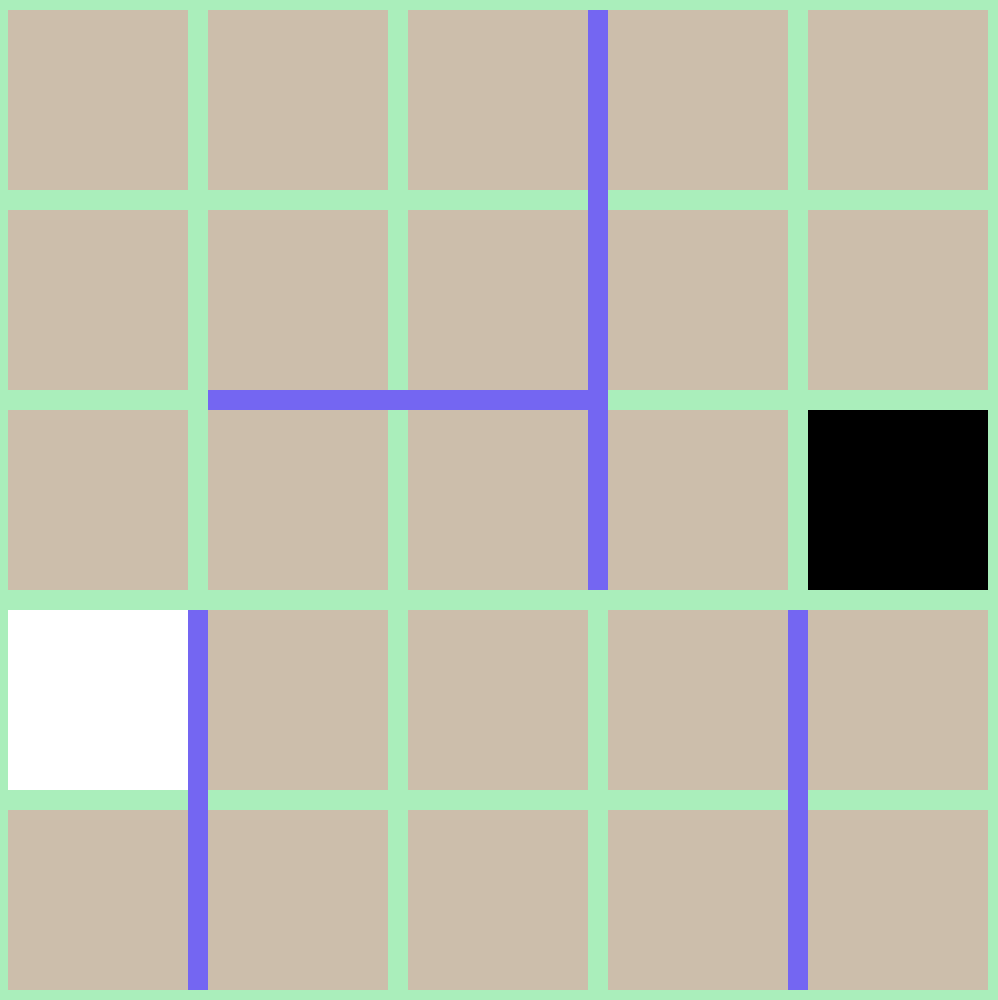
\includegraphics[width=0.3\textwidth]{figures/state-str.png}
    \caption{Board representation of the state given in equation \ref{eq:state-str}}
    \label{fig:state-str}
\end{figure}

\subsection{User interface}
In order to visualize and play games abstracted by the aforementioned logic, we provide a user interface with parameters that can be tuned according to the chosen configuration of the game. To this extent, we used the python \textit{SDL}-based library \textit{PyGame}\cite{pygame}. Our relatively simple yet functional \textit{GUI} is shown in figure \ref{fig:gui}.
\begin{figure}
    \centering
    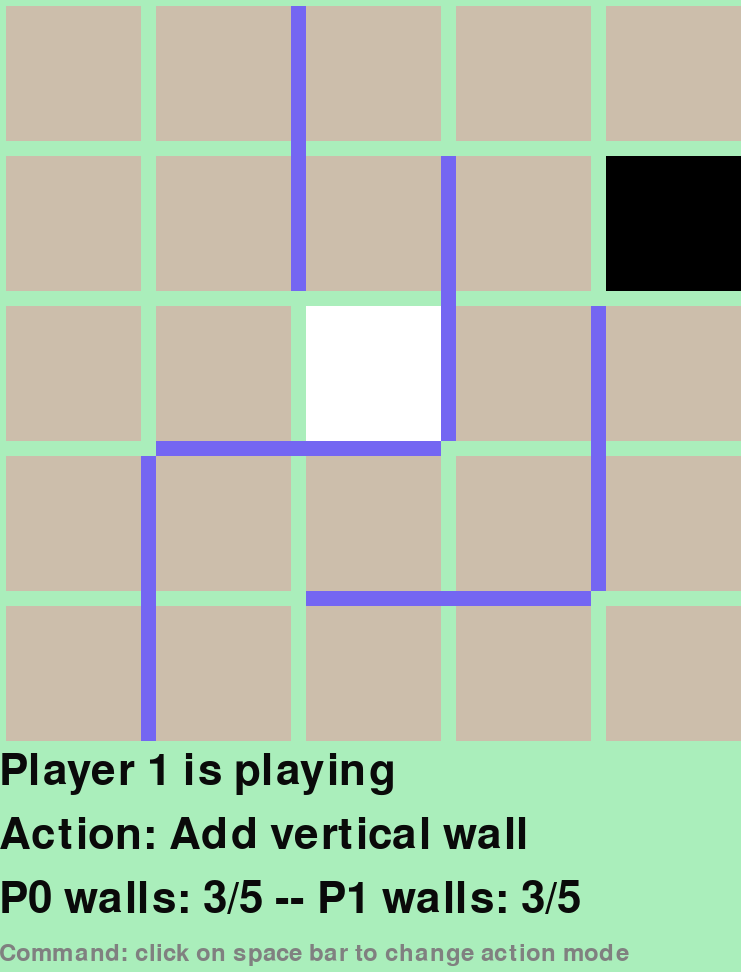
\includegraphics[width=0.3\textwidth]{figures/gui.png}
    \caption{Provided user interface}
    \label{fig:gui}
\end{figure}


\section{Models}
\label{sec:models}

\subsection{MC-RAVE}
In order to solve such a two-player strategy game, MCTS has often been used since it is a classical tree search method \cite{mcts-review}. In particular, MC-RAVE \cite{mc-rave} is an algorithm based on MCTS with an improvement on the value fonction $Q$ which is used. We simulate by self-play $N(s)$ games from state $s$. For a given state $s$ and an action $a$, the classical MCTS value fonction was:
$$Q(s,a) = \frac{1}{N(s,a)} \sum_{i=1}^{N(s)} \mathbf{1}_{i}(s,a)z_i$$
where $N(s)$ is the number of simulations starting from state $s$, $\mathbf{1}_{i}(s,a)$ an indicator function returning 1 if action $a$ was selected in state $s$ during the $i$-th simulation, $N(s,a):=\sum_{i=1}^{N(s)} \mathbf{1}_{i}(s,a)$ the number of simulations in which action $a$ was selected in state $s$, and $z_i$ the final outcome of the $i$-th simulation.

MCTS consists in updating a \textit{search tree}. At each simulation, we use either a \textit{tree policy} or a \textit{default policy} to choose next action. The tree policy is used when the current state is represented in the search tree and it consists in selecting the best child. Otherwise, the default policy is used, what means in our case that we select uniformly at random one action among all possible actions.

The main issue of this algorithm is that it needs a lot of simulations to estimate the value $Q(s,a)$. Rapid Action Value Estimation (RAVE) \cite{mc-rave} tackles this issue by providing a way to quickly estimate the value of an action, thanks to the \textit{all-moves-as-first} (AMAF) heuristic. The main idea is that we suppose each action has a global value, no matter when it is played. So we can estimate the value of an action $a$ in state $s$ as follows:
$$\tilde Q(s,a) = \frac{1}{\tilde N(s,a)} \sum_{i=1}^{N(s)} \mathbf{\tilde 1}_{i}(s,a)z_i$$
where $\mathbf{\tilde 1}_{i}(s,a)$ is an indicator function returning 1 if state $s$ was encountered at any step $t$ of the $i$-th simulation, and action $a$ was selected at any state $u\geq t$, and $\tilde N(s,a):=\sum_{i=1}^{N(s)} \mathbf{\tilde 1}_{i}(s,a)$ the number of simulations used to estimate the AMAF value. So in RAVE algorithm, rather than looking at simulations where action $a$ was selected in state $s$, we look at all simulations where action $a$ was selected \textit{after} state $s$. It is faster to compute, but less accurate.

MC-RAVE \cite{mc-rave} simply consists in a trade-off between previous MCTS and RAVE, by using the following $Q$ value:
$$Q_*(s,a) = (1-\beta(s,a))Q(s,a) + \beta(s,a)\tilde Q(s,a)$$
We use a hand-crafted schedule proposed in the same paper:
$$\beta(s,a) = \sqrt[]{\frac{k}{3N(s)+k}}$$
with $k=1000$.

Finally, we use UCT-RAVE \cite{mc-rave} to give a bonus to exploration:
$$Q_*^+(s,a) = Q_*(s,a) + c\:\:\sqrt[]{\frac{\log N(s)}{N(s,a)}}$$
with $c$ a trade-off parameter.

\subsection{AlphaZero agent}
\label{ssec:alphazero}
    To alleviate the computational burden of tree search, \textit{AlphaZero}\cite{alphazero} proposes to perform MCTS where nodes are expanded thanks to the evaluation of a single policy-value network $f_\theta(s)=(\mathbf{p}, v)$ that takes as input a state $s\in \mathcal{S}$ and provides an action policy $\mathbf{p}\in\mathcal{P}(\mathcal{A})$ (see appendix \ref{sec:alphazero-network}). Similarly to conventional MCTS, each node represents a state and a edge stands for a state-action pair whose attributes are $N(s,a)$ its number of visit, $W(s,a)$ the accumulated action value, $Q(s,a)$ the average action value and $P(s,a)$ the prior probability of this pair. With this setup, we follow iteratively three consecutive steps:
    \begin{enumerate}
        \item \textbf{Search:} we start from an uninitialized tree whose single root node is the current state $s_0$ of the simulation. For every simulation, as long as a leaf as not been reached, the tree is explored by choosing actions according \textit{UCT} (Upper Confidence bounds) algorithm that treats the tree as a multi-armed bandit problem and maximizes an upper confidence bound on the value of actions : $$a_t=\argmax_{a\in\mathcal{A}}(Q(s_t, a)+c_{uct}P(s_t,a)\frac{\sqrt{\sum_{b\in\mathcal{A}}N(s_t, b)}}{1+N(s_t,a)})$$ where $c_{uct}$ enables tuning between greedy exploitation and exploration of the tree.
        \item \textbf{Expansion:} everytime a leaf $s_L$ is encountered in the rollout, it is expanded by adding edges following the estimation provided by the neural network $f_\theta(s_L)=(\mathbf{p_L}, v_l)$ i.e each edge is initialized with $N(s_L, a)=W(s_L,a)=Q(s_L,a)=0$ and $P(s_L,.)=\mathbf{p_L}$.
        \item \textbf{Backup:} the action values and visits of each rollout are back-propagated following $N(s_t, a_t) = N(s_t, a_t) + 1$, $W(s_t, a_t) = W(s_t, a_t) + v$ and $Q(s_t, a_t)=\frac{W(s_t, a_t)}{N(s_t, a_t)}$
    \end{enumerate}


    Unlike \textit{AlphaGo}\cite{alphago} whose expansion was guided by a network trained by supervision on real human-generated data, \textit{AlphaZero} uses self-play schemes to generate training samples without human knowledge which makes it particularly interesting in the context of \textit{Quoridor} for which we have no collected data. We adapted these schemes to our \textit{Quoridor} environment as follows. We first randomly initialize the evaluation network $f_{\theta_0}$ with random weights $\theta_0$ and then proceed iteratively:
    \begin{enumerate}
        \item the last trained network $f_{\theta_i}$ is used to generate self-play games where each move is chosen according to a \textit{MCTS} as described above. More precisely, actions are chosen following the search policy given by the visit counts of the root edges accumulated during the search and tempered with a temperature parameter $\tau$ i.e. $\boldsymbol{\pi}(.|s_0)=\frac{N(s_0,.)^\frac{1}{\tau}}{\sum_{b\in\mathcal{A}}N(s_0, b)^\frac{1}{\tau}}$ and we record state-action-outcome tuples $(s_t, \boldsymbol{\pi}_t, z)$ where $z$ is $1, -1, 0$ respectively for a victory, a defeat or a draw.
        \item the network is $f_{\theta_{i+1}}$ is initialized with the weights of $f_{\theta_i}$ and trained with batches of self-play records sampled by previous models i.e $f_{\theta_i}, f_{\theta_{i-1}}, \ldots$. The idea of the training is to make the network match the \textit{MCTS} search policy $\boldsymbol{\pi}$ and real outcome of the episode $v$ (not the one estimated at the time of the search!). To do so, we use an MSE loss on the value, a cross-entropy loss on the estimated policy and add $L2$ regularization:
        \begin{equation}
            L(\theta) = \underbrace{(z-v)²}_\text{MSE}+\underbrace{\boldsymbol{\pi}^T\log\mathbf{p}}_\text{cross-entropy}+\underbrace{c_{reg}\lVert\theta\rVert_2}_{L2\text{ reg}}
        \end{equation}
    \end{enumerate} 

    \begin{table}[h]
        \centering
        \begin{tabular}{lll}
            \toprule
            & Parameter & Value \\
            \midrule
            \textbf{Game} & Size of the board & 5 \\
            & Maximum number of walls per player & 5 \\
            & Maximum number of turns & 100 \\
            \midrule
            \textbf{Self-play} & Number of games & $1000$ \\
            & Number of \textit{MCTS} simulations & $200$ \\
            & UCT constant $c_{uct}$ & $1.25$ \\
            & Initial temperature & $1.0$ \\
            & Number of tempered steps & $20$ \\
            \midrule
            \textbf{Training} & Learning rate & $1e$-$3$\\
            & Epochs for each iteration & 100 \\
            &Batch size & 32 \\
            &$L2$ regularization parameter $c_{reg}$ & $1e$-$4$ \\
            \midrule
            \textbf{Model} & Number of filters & $128$\\
            & Number of residual blocks & $15$ \\
            \midrule
            \textbf{Evaluation} & Evaluation time & $2$s \\
            \bottomrule
        \end{tabular}
    \caption{Parameters used in our implementation of AlphaZero}
    \label{tab:alphazero-params}
    \end{table}

    Parameters used for the above-mentioned optimization cycle are shown in table \ref{tab:alphazero-params}. The architecture of the estimation network is given in appendix \ref{sec:alphazero-network} and is directly inspired from the work of \cite{alphazero}. More interestingly, it leverages the 2D geometric structure (and thus invariances) of the \textit{Quoridor} board through a 2D state representation. The previously described state space $s_t$ is indeed turned into a \textit{"plane"}-based representation $F_t$ with the following $3$ feature planes:
    \begin{itemize}
        \item a one-hot encoding plane for the current player (i.e. $0$ everywhere and $1$ at the player plosition)
        \item a one-hot encoding plane for the opponent player 
        \item a plane for walls where $0, 1, 2$ respectively stand for empty, horizontal wall and vertical wall (all things considered, it could also be interesting to try two different feature planes for both horizontal and vertical walls). Note that the plane of walls is smaller than the board dimensions; we therefore pad it with $0$s.
    \end{itemize}  
    As the network needs some temporal knowledge of the state, previous state space feature planes $T-1$ are concatenated and a constant feature plane $C_t$ specifying which player is playing (i.e. $0$ for player 0, $1$ for player 1) to provide overall $3\times T + 1$ feature planes: $(F_{t-T+1}, \ldots, F_{t-1}, F_t, C_t)$. In order for the representation to be consistent and for the network to capture the dynamics at play, the concatenated feature planes are then rotated (180°) to match the perspective of the current player. Finally, actions are mapped to indices which means that the features abstracted by the convolutional layers are flattened to obtain the policy vector $\mathbf{p}$ (see appendix \ref{sec:alphazero-network}) for more details.
    
    In evaluation mode, a time parameter can be given and limit the model to human-like evaluation conditions (i.e. tree searches will be performed as long as the agent can do it).


\section{Results and Discussion}
\label{sec:results}

\subsection{MC-RAVE}
For this draft version of the paper, we don't have final results to present. We trained our agent by self-play, as described above, with parameters $k=1000$ and $c=0.1$. Next step will be to evaluate the performance of such a trained agent.

\subsection{AlphaZero}


\section{Conclusions}
\label{sec:conclusion}

Future works:
- Use importance sampling on episode records as suggested in Mu-zero paper
- Equivariant action space
- Add constraint to deter the agents from placing walls initially (as of now, they are equally weighted and this is very unstable during training = agents tend to place all their walls at the beginning thus making no use of them)
- use dilated convolutions? (capture on a more global scale)

\bibliographystyle{plain}
\bibliography{biblio}

\newpage
\section*{AlphaZero network configuration}
\label{sec:alphazero-network}
Even though our \textit{AlphaZero}-like network is close to the one initially proposed in \cite{alphagozero}, we chose smaller parameters due to the reduced size of our game space (see table \ref{tab:alphazero-params} for more details). Our implementation uses \textit{PyTorch}\cite{pytorch} and consists in:
\begin{itemize}
    \item a first convolution of $128$ filters of kernel size $3$ with stride $1$ + 2D batch normalization + ReLU activation layer
    \item a stack of residual blocks made of:
    \begin{itemize}
        \item a convolution of $128$ filters of kernel size $3$ with stride $1$ + 2D batch normalization + ReLU activation
        \item a convolution of $128$ filters of kernel size $3$ with stride $1$ + 2D batch normalization + \textbf{a residual connection} + ReLU activation
    \end{itemize}
    \item two output heads:
    \begin{enumerate}
        \item a \textbf{policy head} made of:
            \begin{itemize}
                \item a convolution of $2$ filters of kernel size $1$ with stride $1$ + 2D batch normalization + ReLU activation
                \item a flattener
                \item a dense layer + softmax output layer
            \end{itemize}
        \item a \textbf{value head} made of:
            \begin{itemize}
                \item a convolution of $1$ filter of kernel size $1$ with stride $1$ + 2D batch normalization + ReLU activation layer
                \item a flattener
                \item a dense layer of size $256$ + ReLU activation
                \item a dense layer to output size $1$ + $\tanh$ activation which restricts the output value in $[-1,1]$
            \end{itemize}
    \end{enumerate}
\end{itemize}
Note that each convolution is padded with 0 in order to give the same output size as the input.

\end{document}
